% CURRENT FULL-PANEL WORKING DRAFT, 2026-10-15. Author-facing notes.
% Development manuscript, not a completed submission or success claim.
% Remaining gates: independent outer assessment, optimizer-seed replication,
% matched-input/budget attribution, original-paper benchmarks, full-panel
% ARGformer and external comparators, cross-domain evidence, novelty review.
% H043 completed results are included only as a compact control appendix.
% Root confirmed H043 completion. H044 results remain excluded.
% No original-paper reproduction, universal ranking, novel-operator,
% significance, held-out-test, or real-data PCA claim is supported.
% Root must compile/render, check 6--8 main pages and <=20 total pages.
% No compilation or installation performed by this author.
% Official AuthorKit27 header uses draft mode for internal working use.
\documentclass[letterpaper]{article}
\usepackage[draft]{aaai2027}
\usepackage[hyphens]{url}
\usepackage{graphicx}
\urlstyle{rm}
\def\UrlFont{\rm}
\usepackage{natbib}
\usepackage{caption}
\usepackage{amsmath}
\usepackage{amssymb}
\usepackage{booktabs}
\usepackage{tikz}
\usetikzlibrary{arrows.meta,positioning}
\frenchspacing
\pdfinfo{/TemplateVersion (2027.1)}
\setcounter{secnumdepth}{2}
\title{Whole-Tree Message Passing with Local Clade-Change Features\\
for Ancestry Inference}
\author{Anonymous Authors}
\affiliations{}
\begin{document}
\maketitle
\begin{abstract}
Changing inferred genealogies provide a structured representation for local ancestry prediction, but strong span accuracy can conceal poor tract boundaries. We study a whole-tree graph neural pipeline on a common panel of 476 diploids, with 32 training and eight development validation simulations. The model encodes observed SNPs and known reference annotations, performs PyTorch Geometric message passing over every native tree, and processes all sampled haplotypes with a bidirectional genomic GRU. A local adapter marks exact sampled-leaf clades gained or lost between adjacent trees. On the present-day cohort, this model attains $96.5778\pm0.5954\%$ span accuracy, compared with $94.4461\pm1.1491\%$ for the current native ARGMix pipeline. The difference includes input, training and selection effects. Under matched added training and parameter count, local flags exceed a tensor clade-event model by 0.3104 percentage points, whereas tensor coupling exceeds its event-MLP control by only 0.0667 points. Boundary F1 remains $18.05\pm1.84\%$ at 1\,kb tolerance. These development results favor the simpler local structural features within the examined family and identify transition recognition and readout resolution as unresolved limitations.
\end{abstract}

\section{Introduction}
Local ancestry inference assigns source-population labels along a sampled genome. A genealogy can organize evidence from many reference and query haplotypes, while its changes along the genome describe a second source of structure. These two axes pose different modeling problems. Within a marginal tree, information must travel between known references and queries through anonymous inferred ancestors. Across trees, sampled haplotypes persist while internal nodes and descendant clades change.

Recent ancestry systems motivate learning from genealogical structure. AncestralPaths accompanies a demographic analysis of ancient Eurasians \citep{eurasians2024}. ARGMix uses graph-transformer representations and genomic sequence modeling \citep{ancientancestry2026}. ARGformer learns path representations and performs native retrieval \citep{argformer2026}. Their released representations, supervision and prediction rules differ. A comparison on common observations therefore needs both a common scoring endpoint and an explicit account of the remaining pipeline differences.

We investigate a compact whole-tree model that retains all 952 observed haplotypes and every inferred marginal tree. Its graph computation uses PyTorch Geometric \citep{pyg2019}. A bidirectional GRU \citep{gru2014} models the complete sequence of tree contexts for each sampled haplotype. Observed SNP features and reference annotations enter the graph encoder directly. Predictions do not consume another ancestry model's outputs.

The empirical question is whether extra machinery for coupling changing clades is useful beyond simpler structural features. We compare a tensor interaction and a matched event MLP over the same clade-event inputs, then examine a local flag adapter with the same additional parameter count and training budget. The local adapter uses only a node's own first-sweep state and two observation-derived flags. It does not gather a neighboring tree's learned state. This distinction permits an interpretable comparison between a richer interaction and local structural conditioning.

The completed results support three findings. First, the local-flag model has the highest present-day mean span accuracy among these completed development conditions. Second, the tensor interaction adds only a small observed difference over its matched event MLP, and the local control exceeds both. The results do not establish a distinct new neural operator. Third, high span accuracy coexists with weak tract-boundary prediction. A fixed-output diagnostic separates missing candidate boundaries from errors at boundaries the decoder could express.

The study uses independent simulations as the unit of partitioning and reporting. Its eight validation simulations also support checkpoint selection and architecture development. The reported variation is across those simulations from one optimizer seed per condition. Independent confirmation, broader comparators and a completed novelty assessment remain necessary before stronger claims.

\section{Task and Evaluation Protocol}
\subsection{Observed Panel and Simulation Split}
The common panel contains 476 diploids, or 952 phased haplotypes. There are 686 query haplotypes and 266 pure-reference haplotypes. Queries comprise present-day individuals (182 haplotypes), Bronze Age (162), BAA (14), Neo (302) and Yam (26). The reference panel comprises WHG (102), EHG (86), Ana (50) and CHG (28). Cohort names follow the released roster. In particular, Bronze Age is only an approximate correspondence to the ARGMix paper's Post-Neolithic category.

Each independent simulation spans 2\,Mb. The completed development data contain 32 TRAIN and eight VAL simulations. Simulation identity is assigned before downstream windows, sampled rows or genomic chunks are constructed. Thus nearby trees from a single simulation do not enter different partitions. An independent outer assessment is outside the results reported here.

The simulation condition follows the released ancient-European demographic and sample-panel definition, with a uniform recombination rate of $10^{-8}$ and mutation rate of $1.25\times10^{-8}$ per base per generation. Current msprime \citep{msprime2022} settings use the Hudson ancestry model, discrete coordinates and JC69 mutations. Genealogies used by the present full-panel models are native Relate post-population-size reconstructions \citep{relate2019}. Reused source-module names containing \emph{tsinfer} do not identify the topology actually read in this experiment.

Observed inputs include phased genotypes, inferred topology and branch ages, sample ages and roles, and known reference-source classes. Query ancestry annotations are external supervision. Census labels, truth breakpoints and query-source labels do not define the model's observed feature bank, genomic holds or evaluation coordinates. Reference labels are available to every applicable native adapter as observed panel annotations.

\subsection{Common Four-Class Endpoint}
The shared endpoint has class order Ana, CHG, WHG and EHG, denoted C4. The native AncestralPaths classifier produces six path probabilities. For the common endpoint we collapse them before choosing a class,
\begin{equation}
(p_{\mathrm{Ana}},p_{\mathrm{CHG}},p_{\mathrm{WHG}},p_{\mathrm{EHG}})
=(p_1+p_5,p_2+p_6,p_3,p_4).
\end{equation}
Its native six-path SNP-focal endpoint remains separate. This mapping defines the present comparison and does not reconstruct a separately trained model from a published table.

Scoring uses the same original 100\,bp center-bin support for every pipeline. Bins are clipped to inferred coverage. Missing support is not filled and uncovered tails are not extrapolated. Truth intervals are intersected with these fixed bins to obtain exact class-specific physical mass. Let $m_{iqc}$ be the represented base-pair mass of class $c$ for bin $i$ and query $q$, and let $p_{iqc}$ be a model probability. For a cohort $Q$,
\begin{align}
A_Q&=\frac{\sum_{i,q\in Q,c}m_{iqc}
 \mathbf{1}\{c=\arg\max_k p_{iqk}\}}
 {\sum_{i,q\in Q,c}m_{iqc}},\\
\mathrm{NLL}_Q&=-\frac{\sum_{i,q\in Q,c}m_{iqc}\log p_{iqc}}
 {\sum_{i,q\in Q,c}m_{iqc}}.
\end{align}
Zero probability on positive true-class mass yields infinite NLL. We apply no probability floor, post-hoc renormalization, purity filter or fitted calibration.

The primary endpoint is equal-simulation mean accuracy for the 182 present-day query haplotypes. All-query, ancient-query and individual-cohort results are secondary. We report sample SD with divisor $8-1$ across the eight independent VAL simulations. These SDs describe simulation variation for the fitted models, rather than optimizer-seed uncertainty or confidence intervals. Primary selection scores retain their registered FP32 arithmetic. Broader diagnostics integrate physical spans in FP64 and agree at the displayed precision.

\section{Whole-Tree Model with Local Clade Flags}
Let $T_t$ denote the inferred tree on genomic hold $I_t$, with the same ordered set of sampled haplotypes in every tree. Internal-node indexes are local to a tree. The model makes a C4 probability vector for every query on each native hold. Figure~\ref{fig:architecture} shows the implemented data flow.

\subsection{Observed SNP and Node Encoding}
For each SNP and sampled haplotype, the site encoder receives 19 observed channels: eight logged donor allele-frequency values for its called allele, eight availability masks, the log panel frequency of that allele, site entropy and a call indicator. Missing calls are masked. A $19\to32\to32$ MLP with GELU and tanh transforms each tuple. Within each native hold, the encoder pools the mean and coordinatewise maximum, then appends log call count, an empty-pool indicator and log hold span. A $67\to32$ projection produces a sampled-leaf SNP representation.

Known donor labels enter as a four-class one-hot vector. Query labels are masked and accompanied by an unknown-label indicator. The leaf representation also receives normalized log sample age. A $38\to32$ projection combines these six annotations with the SNP encoding. Every graph node receives a separate projection of normalized log node age, root status and sampled-node status. The sampled-leaf feature is added only at its own native node.

Two sigmoid gates, one for each message direction, are computed from nine observed edge channels. These combine inferred edge geometry with mutation-concordance summaries. All graph states have width 32. This encoding keeps known reference annotations distinct from the query targets used by the external loss.

\subsection{Upward Messages and Recipient Exclusion}
Each tree sweep uses actual PyG \texttt{MessagePassing} and \texttt{SumAggregation} calls. Let $b_v$ be a node's encoded base feature, $g^\uparrow_u$ its upward gate and $d_v$ the number of children of $v$. The upward messages and state have the form
\begin{align}
m_{u\to v}&=\frac{g^\uparrow_u\odot W_\uparrow h_u}{\max(1,d_v)},\\
s_v&=\sum_{u\in\mathrm{child}(v)}m_{u\to v},\\
h_v&=\mathrm{LN}\!\left(b_v+
 \tanh\!\left(A_\uparrow[b_v,s_v]+a_\uparrow\right)\right).
\end{align}
Native topological levels determine evaluation order. The exact transformed upward contribution of every child is retained for the downward sweep.

For a nonroot node $u$ with parent $v$, the downward context excludes that child's own upward contribution,
\begin{equation}
c_{v\setminus u}=o_v+b_v+s_v-m_{u\to v}.
\end{equation}
A gated linear transformation, learned downward update, tanh and layer normalization map this context to $o_u$. Roots start with zero outside state. The sampled-leaf context is a learned width-32 projection of the concatenated upward and outside states. Both sweeps traverse every native node. They neither select a fixed ancestor depth nor replace the tree with a query-reference subgraph.

\begin{figure*}[t]
\centering
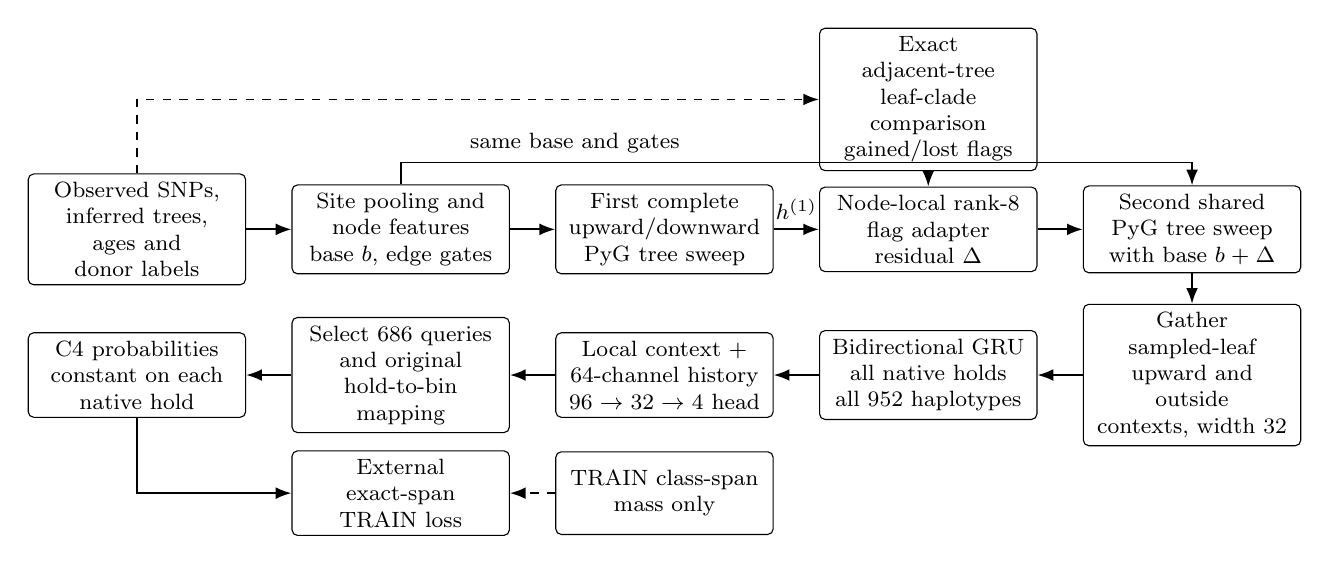
\begin{tikzpicture}[
 block/.style={draw,rounded corners=2pt,align=center,text width=2.55cm,
 minimum height=1.05cm,inner sep=3pt,font=\footnotesize},
 flow/.style={-{Latex[length=2mm]},line width=.65pt},
 observed/.style={flow,dashed}]
\node[block] (obs) at (0,0) {Observed SNPs,\\inferred trees,\\ages and donor labels};
\node[block] (base) at (3.35,0) {Site pooling and\\node features\\base $b$, edge gates};
\node[block] (first) at (6.7,0) {First complete\\upward/downward\\PyG tree sweep};
\node[block] (local) at (10.05,0) {Node-local rank-8\\flag adapter\\residual $\Delta$};
\node[block] (second) at (13.4,0) {Second shared\\PyG tree sweep\\with base $b+\Delta$};
\node[block] (flags) at (10.05,1.65) {Exact adjacent-tree\\leaf-clade comparison\\gained/lost flags};
\node[block] (leaves) at (13.4,-1.85) {Gather sampled-leaf\\upward and outside\\contexts, width 32};
\node[block] (gru) at (10.05,-1.85) {Bidirectional GRU\\all native holds\\all 952 haplotypes};
\node[block] (head) at (6.7,-1.85) {Local context +\\64-channel history\\$96\to32\to4$ head};
\node[block] (queries) at (3.35,-1.85) {Select 686 queries\\and original\\hold-to-bin mapping};
\node[block] (prob) at (0,-1.85) {C4 probabilities\\constant on each\\native hold};
\node[block] (loss) at (3.35,-3.35) {External exact-span\\TRAIN loss};
\node[block] (truth) at (6.7,-3.35) {TRAIN class-span\\mass only};
\draw[flow] (obs)--(base);
\draw[flow] (base)--(first);
\draw[flow] (first)--node[above,font=\footnotesize] {$h^{(1)}$}(local);
\draw[flow] (local)--(second);
\draw[observed] (obs.north)--(0,1.65)--(flags.west);
\draw[observed] (flags)--(local);
\draw[flow] (base.north)--(3.35,.85)--node[above,pos=.22,font=\footnotesize] {same base and gates}(13.4,.85)--(second.north);
\draw[flow] (second)--(leaves);
\draw[flow] (leaves)--(gru);
\draw[flow] (gru)--(head);
\draw[flow] (head)--(queries);
\draw[flow] (queries)--(prob);
\draw[flow] (prob.south)--(0,-3.35)--(loss.west);
\draw[observed] (truth)--(loss);
\end{tikzpicture}
\caption{Actual H042 computation. The two full-tree sweeps share learned weights. Only the first upward states feed the local adapter. Dashed arrows supply structural flags or external training supervision. Adjacent trees contribute exact clade-presence flags, without transferring learned node states through the adapter. The genomic GRU processes the complete observed sequence. Query truth never enters the forward feature path. Architecture provenance is E6--E7 in Appendix~\ref{app:provenance}.}
\label{fig:architecture}
\end{figure*}

\subsection{Exact Local Clade-Change Flags}
For an internal node $v$, let $C_t(v)$ be its set of descendant sampled haplotypes. A proper clade contains more than one and fewer than 952 sampled leaves. The structural preparation compares these sets exactly between adjacent trees using temporary integer bitsets. Equal proper clades on unary chains use the deepest structural representative. Leaf and root clades are excluded.

A representative receives a gained flag $g_v$ if its proper clade is absent from the preceding tree and a lost flag $\ell_v$ if absent from the following tree. The corresponding missing-neighbor flags at sequence ends remain zero. Only two compact flags per native node are retained. Exact bitsets are not neural features and no ancestral-node correspondence is asserted. In particular, an identical sampled-leaf clade is a structural statement, rather than proof that two inferred internal nodes are the same biological ancestor.

The H042 adapter operates on a node's own first upward state $h_v^{(1)}$,
\begin{equation}
\Delta_v=O\!\left[
g_v(Uh_v^{(1)}\odot Vh_v^{(1)})
-\ell_v(Uh_v^{(1)}\odot Wh_v^{(1)})\right].
\label{eq:local}
\end{equation}
Here $U,V,W:\mathbb{R}^{32}\to\mathbb{R}^{8}$ and
$O:\mathbb{R}^{8}\to\mathbb{R}^{32}$ are bias-free. Their 1,024 weights increase the body from 29,764 to 30,788 parameters. The output projection $O$ starts at zero. A second complete tree sweep uses $b_v+\Delta_v$ with the original gates and the same sweep weights. Fresh state buffers are used for this second traversal.

Equation~\ref{eq:local} contains no other node's or tree's latent state. It is a local structural-feature control for the more elaborate clade-event interactions, not a claimed novel message-passing primitive.

\subsection{Complete Genomic History and Readout}
The second-sweep leaf contexts are concatenated with three observed geometry channels: log hold span and log distances to the preceding and following hold midpoints. The normalization denominator is $\log(2{,}000{,}001)$. A single-layer bidirectional GRU receives the resulting 35-channel sequence, with hidden width 32 in each direction. It processes all native holds for all 952 sampled haplotypes.

The classifier concatenates the local 32-channel context and 64-channel recurrent history. A $96\to32\to4$ MLP with GELU yields C4 logits. Only afterward does the readout select the 686 queries and map each original scored bin to its native hold. Consequently the current prediction is constant within a hold. SNP chunks of 256 are a memory strategy for exact pooling, not truncated recurrent histories or independent genomic training examples.

This construction combines established graph propagation, local structural features and recurrent sequence modeling. Temporal graph state-space methods provide a related perspective on persistent sampled interfaces \citep{graphssm2024}. The present empirical comparisons evaluate these concrete implementations and do not resolve priority across the broader literature.

\section{Training and Comparator Conditions}
\subsection{Whole-Parent Optimization}
The training objective uses all 686 query haplotypes. Because logits are constant on a native hold, class-specific target spans from every original scored bin can be summed by hold without changing the physical-span cross-entropy objective. For hold $t$,
\begin{equation}
M_{tqc}=\sum_{i:\,r(i)=t}m_{iqc},
\qquad
\mathcal{L}=-\frac{\sum_{tqc}M_{tqc}\log p_{tqc}}{\sum_{tqc}M_{tqc}}.
\end{equation}
This aggregation preserves every represented target span. It does not sample trees or discard query states. Targets remain external to the observed bank.

The H038 aligned body and its zero-concordance control each complete 30 FP32 passes, or 960 whole-simulation optimizer updates. The zero-concordance arm sets the first three branch-support channels to zero. It retains SNP inputs, topology, remaining support summaries and the complete GRU. Thus it is a particular routing-feature ablation, not an SNP-free or genealogy-free comparator.

H040 tensor and event-MLP conditions and H042 flags begin from the same selected H038 aligned checkpoint. Each completes 30 additional passes and 960 additional updates. AdamW is reset with learning rate $10^{-3}$, weight decay $10^{-4}$, betas $(0.9,0.999)$ and epsilon $10^{-8}$. Gradient norm is clipped at 1. These extensions have 30,788 parameters and use optimizer seed 101. The same added budget does not make their total exposure equal to the unextended H038 body.

Checkpoints at five-pass intervals are evaluated using equal-simulation present-day VAL accuracy, with the registered NLL and earlier-pass tie breaks. The selected aligned H038 checkpoint is pass 30, while zero concordance selects pass 25 although both finish pass 30. H040 and H042 select additional pass 30. VAL labels do not supply optimization gradients, but repeated development and selection on this split limit confirmatory interpretation.

\subsection{Matched Interactions and Native Baselines}
The H040 comparison holds its clade-event inputs, initialization protocol, 1,024 added weights and additional update budget fixed between a tensor interaction and an event MLP. Both route signed residuals through changed-clade event incidences, followed by the second shared tree sweep. The local H042 control uses the same size and added budget but substitutes the two exact local flags in Equation~\ref{eq:local}. It therefore asks whether those event interactions are needed beyond local topology-change information.

Native AncestralPaths retains the released Keras Dense512 classifier, six path outputs and fixed five-epoch training. Its actual fit uses 5,190,874 sampled rows from the 32 TRAIN simulations and selects final epoch 5. This is the executable released Dense model, not a reconstruction of a published CNN. Its derived C4 probabilities are scored without changing the native model.

Current native ARGMix retains its author implementation, with disclosed full-panel slot and metadata adaptation. It uses the released 15-reference representation without ancestor features and the native genomic sequence model. Its fit uses source seed 50 and selects epoch 9 by the original smoothed, masked, unweighted VAL batch-mean loss. Native patience is 2 with a 20-epoch cap. External full-support scoring does not replace that inner selection rule.

These conditions share simulation observations and physical scoring support, but they do not isolate architecture. The whole-tree model additionally consumes observed SNP features. Native row sampling, reference representations, sequence chunks, supervision, training exposure and checkpoint objectives remain method-specific. H040 and H042 also receive an additional 960 updates after the H038 warm start. Their comparison with the native pipelines is a development pipeline comparison.

\section{Results}
\subsection{Primary Span Accuracy}
Table~\ref{tab:primary} gives the completed present-day results. H042 local flags attain $96.5778\pm0.5954\%$, compared with $95.4891\pm0.8338\%$ for the H038 aligned body and $94.4461\pm1.1491\%$ for current native ARGMix. The H042--ARGMix difference is 2.1317 percentage points. This is an observed difference between the specified fitted pipelines, with the input, optimization and selection qualifications above.

\begin{table}[t]
\centering
\small
\begin{tabular}{lrr}
\toprule
Condition & Accuracy (\%) & Mean NLL \\
\midrule
Native AP (C4) & $93.7830\pm0.8385$ & $\infty$ \\
Current native ARGMix & $94.4461\pm1.1491$ & 0.219695 \\
H038 zero concordance & $94.9252\pm0.7917$ & 0.147232 \\
H038 aligned & $95.4891\pm0.8338$ & 0.133497 \\
H040 event MLP & $96.2007\pm0.7048$ & 0.110014 \\
H040 tensor & $96.2674\pm0.7493$ & 0.109332 \\
H042 local flags & $96.5778\pm0.5954$ & 0.100656 \\
\bottomrule
\end{tabular}
\caption{Present-day development span accuracy, mean$\pm$sample SD across eight simulations. All models use one optimizer seed. NLL has no probability floor. Native AP is the derived C4 endpoint. H040/H042 have 960 additional updates beyond the H038 warm start. Provenance: E1--E5 and E11, Appendix~\ref{app:provenance}.}
\label{tab:primary}
\end{table}


The aligned H038 body exceeds zero concordance by 0.5639 percentage points at the selected checkpoints. Both runs complete 960 updates, but their selected passes differ. This result supports retaining the observed concordance features in this development condition. It does not identify an effect of all SNP information, all genealogy information, or PyG software alone.

The same caution applies to the extension's improvement over the H038 body. H042 changes capacity and performs two shared tree sweeps, then trains for another 960 updates. Its difference from the base score cannot be attributed entirely to the flag mechanism. The closer comparisons are the H040 tensor, H040 event-MLP and H042 local-flag conditions, which have the same added count and budget.

Native AncestralPaths has finite accuracy but infinite strict raw FP32 NLL on the primary cohort. One simulation places zero probability on the true class over 800 query-base pairs. We preserve this result rather than floor probabilities, exclude the simulation or silently average only finite NLLs. Accuracy and NLL measure different aspects of a prediction distribution.

\subsection{Local Flags Versus Clade-Event Interactions}
Table~\ref{tab:paired} reports paired present-day differences across the same eight simulations. Tensor coupling exceeds its matched event MLP by a mean 0.0667 percentage points, with positive differences in six of eight simulations. H042 local flags exceed the tensor condition by 0.3104 points and the event MLP by 0.3771 points, with positive differences in each of the eight simulations for these fitted models.

\begin{table}[t]
\centering
\small
\begin{tabular}{lrr}
\toprule
Paired comparison & Difference (pp) & Positive \\
\midrule
Tensor $-$ event MLP & $0.0667\pm0.0886$ & 6/8 \\
Flags $-$ tensor & $0.3104\pm0.2588$ & 8/8 \\
Flags $-$ event MLP & $0.3771\pm0.2165$ & 8/8 \\
\bottomrule
\end{tabular}
\caption{Equal-simulation paired accuracy differences, mean$\pm$sample SD. Positive counts are descriptive. Both added parameter count and update budget are matched. Provenance: E2--E3.}
\label{tab:paired}
\end{table}


These descriptive comparisons favor the simpler local condition within the examined family. They do not establish that clade-event coupling is generally ineffective. Different incidence definitions, objectives, training conditions or independent simulations could change the result. The present evidence also does not justify attributing a distinct scientific contribution to the tensor interaction itself.

\subsection{Cohort Dependence}
Table~\ref{tab:cohorts} reports all registered cohorts, including the small BAA and Yam groups. H042 has a higher mean span accuracy than the current native AP and ARGMix pipelines in each listed cohort. Across all 686 queries it reaches $98.64\pm0.26\%$, while present-day accuracy is lower at $96.58\pm0.60\%$. The aggregate is therefore not interchangeable with the primary endpoint.

\begin{table*}[t]
\centering
\small
\begin{tabular}{lrrrrr}
\toprule
Cohort & Queries & Native AP (C4) & Current native ARGMix & H038 aligned & H042 local flags \\
\midrule
Present & 182 & $93.78\pm0.84$ & $94.45\pm1.15$ & $95.49\pm0.83$ & $96.58\pm0.60$ \\
Bronze Age & 162 & $94.76\pm1.18$ & $97.71\pm0.75$ & $98.17\pm0.80$ & $99.07\pm0.32$ \\
BAA & 14 & $96.94\pm1.32$ & $98.44\pm1.02$ & $98.90\pm0.89$ & $99.02\pm1.07$ \\
Neo & 302 & $97.57\pm0.27$ & $99.30\pm0.26$ & $99.41\pm0.13$ & $99.53\pm0.18$ \\
Yam & 26 & $95.43\pm1.41$ & $99.22\pm0.90$ & $98.96\pm1.31$ & $99.86\pm0.19$ \\
Ancient & 504 & $96.54\pm0.32$ & $98.76\pm0.31$ & $98.98\pm0.32$ & $99.39\pm0.16$ \\
All queries & 686 & $95.81\pm0.45$ & $97.61\pm0.50$ & $98.05\pm0.43$ & $98.64\pm0.26$ \\
\bottomrule
\end{tabular}
\caption{Cohort span accuracy (\%), mean$\pm$sample SD over eight independent development simulations. Queries counts haplotypes. Ancient and all-query rows are aggregates of the preceding cohorts. BAA and Yam remain explicit despite small sizes. Bronze Age is not asserted to be identical to the published Post-Neolithic panel. Provenance: E1, E4--E5.}
\label{tab:cohorts}
\end{table*}


The contemporary-versus-ancient contrast reflects different query distributions under this demographic condition. Query cohorts differ in ages, source mixtures, tract structure and numbers of haplotypes. These results do not measure performance on an empirical ancient-DNA collection or establish robustness to observation error. Small cohorts also have sparse transition counts, so a high span score does not guarantee a stable boundary estimate.

Advantages are not uniform within the extended neural family. H040 tensor has BAA accuracy $99.14\%$, compared with H042's $99.02\%$. The event MLP has Neo accuracy $99.56\%$, compared with H042's $99.53\%$. Appendix~\ref{app:matched} gives their simulation SDs. The primary ranking thus summarizes a particular registered endpoint rather than dominance on every cohort and metric.

\subsection{High Span Accuracy, Weak Boundaries}
Table~\ref{tab:boundaries} uses the unchanged one-to-one positional boundary matcher at 1\,kb tolerance. H042 improves mean F1 to $18.05\pm1.84\%$, but its recall is only $22.30\pm1.86\%$ and precision is $15.21\pm2.01\%$. Accurate long tracts can dominate physical-span accuracy while numerous missed and extra transitions remain.

\begin{table}[t]
\centering
\small
\begin{tabular}{@{}lrrr@{}}
\toprule
Condition & Prec. & Recall & F1 \\
\midrule
Native AP (C4) & $3.95\pm0.48$ & $32.36\pm2.06$ & $7.03\pm0.78$ \\
ARGMix & $9.16\pm1.49$ & $16.41\pm2.22$ & $11.74\pm1.73$ \\
H038 aligned & $10.71\pm1.21$ & $17.99\pm2.01$ & $13.42\pm1.47$ \\
H042 flags & $15.21\pm2.01$ & $22.30\pm1.86$ & $18.05\pm1.84$ \\
\bottomrule
\end{tabular}
\caption{Present-day boundaries at 1\,kb tolerance (\%), mean$\pm$sample SD across eight simulations. The positional matcher ignores transition class identity. Provenance: E1, E4--E5 and E8.}
\label{tab:boundaries}
\end{table}


Native AP has higher boundary recall than H042 in this comparison, accompanied by much lower precision. H042's larger F1 consequently should not be read as an improvement in every transition metric. For H042 the pooled counts are 4,008 true changes, 5,920 predicted changes and 892 positional matches. These pooled event counts are distinct from the equal-simulation means and SDs in the table.

A separate fixed-output H038 diagnostic clarifies two limitations. Of 4,008 true changes, 1,094, or 27.30\%, have no allowed native-hold readout edge within 1\,kb. Its class-agnostic hold-edge oracle recall is $72.70\pm2.80\%$. Yet 2,195 of the aligned model's 3,289 missed boundaries still have a nearby candidate. Missing readout resolution therefore explains only part of the recognition deficit.

False internal ancestry islands of at most 10\,kb account for $35.46\pm2.71\%$ of H038's extra boundaries, while all predicted tracts of that length contain only $3.83\pm0.73\%$ of wrong query-base pairs. Event counts and wrong physical mass emphasize different errors. This diagnostic concerns the frozen H038 outputs and is not an H042 island analysis. It motivates prospective continuity and finer-readout comparisons without selecting a smoothing rule on these VAL results.

\subsection{Observed Training Cost}
The completed aligned H038 run records 43.6 seconds per 32-simulation pass, 1,307.9 seconds in training and 1,698.5 seconds total elapsed time. Its peak CUDA allocated memory is 21.35\,GB and reserved memory is 37.16\,GB in decimal units. These are measurements of that training path, excluding full data preparation and external baseline evaluation. They neither isolate a PyG speedup nor establish the cost of H042 or the other complete pipelines.

\section{Discussion and Scope}
The results distinguish representation usefulness from a claim of architectural invention. Local changes in exact sampled-leaf clades are useful features in the present completed comparison. A node-local multiplicative adapter exceeds the examined clade-event interactions under matched added capacity and training. Established tree propagation and a full genomic recurrent model remain essential parts of the concrete system being evaluated. These results leave a simpler structural explanation viable.

Several limitations determine how the scores should be used. The VAL simulations have informed model selection and architecture development. A single optimizer seed cannot quantify training instability. The native comparators preserve their released methods but differ in input evidence, training units, reference choices and selection objectives. The simulated roster and the derived C4 endpoint also differ from the published ARGMix benchmark, which uses different panel, reference and evaluation conditions. Numerical comparisons with its published tables would require a separately verified recipe.

The task is conditional on one demographic simulation family and inferred observation pipeline. A high cohort mean does not establish robustness to genotype errors, demographic misspecification, a different reference panel or real genomes. Full-panel ARGformer, broader external baselines and cross-domain experiments remain outside the completed evidence here. A literature assessment must also separate established components from any defensible distinct contribution before a novelty claim is formulated.

Boundary performance is a substantive remaining weakness. Improving the ability to express a transition inside a native hold addresses a geometric restriction, while improving transition recognition addresses failures where a suitable edge already exists. Neither follows automatically from higher span accuracy. Future evaluation should preserve the fixed physical-support scorer, count real short tracts, and use independent simulations for confirmation rather than tune a post-processing rule on the current boundary errors.

\section{Conclusion}
A compact whole-tree PyG and genomic-GRU pipeline with exact local clade-change flags reaches $96.5778\pm0.5954\%$ present-day span accuracy on eight development simulations. The local feature control exceeds the examined tensor and event-MLP extensions under matched added capacity and training. The completed comparison supports this concrete implementation choice, while weak boundary F1 and pipeline confounds limit broader interpretation. Independent assessment and matched external benchmarking remain necessary.

\bibliography{current_full_panel_refs}

\appendix
\section{Matched Cohort Results}
\label{app:matched}
\begin{table}[t]
\centering
\small
\begin{tabular}{lrrr}
\toprule
Cohort & Event MLP & Tensor & Local flags \\
\midrule
Present & $96.20\pm0.70$ & $96.27\pm0.75$ & $96.58\pm0.60$ \\
Bronze Age & $98.82\pm0.44$ & $98.83\pm0.47$ & $99.07\pm0.32$ \\
BAA & $99.11\pm0.92$ & $99.14\pm0.89$ & $99.02\pm1.07$ \\
Neo & $99.56\pm0.12$ & $99.52\pm0.16$ & $99.53\pm0.18$ \\
Yam & $99.76\pm0.24$ & $99.72\pm0.30$ & $99.86\pm0.19$ \\
Ancient & $99.32\pm0.17$ & $99.30\pm0.21$ & $99.39\pm0.16$ \\
All queries & $98.49\pm0.29$ & $98.49\pm0.34$ & $98.64\pm0.26$ \\
\bottomrule
\end{tabular}
\caption{Matched extended-family cohort span accuracy (\%), mean$\pm$sample SD over eight VAL simulations. Provenance: E2--E3 and E5.}
\label{tab:matchedcohorts}
\end{table}

The same added budget and parameter count do not imply identical cohort rankings. These descriptive results supplement the registered present-day endpoint and do not redefine it.

\section{Completed Neighbor-State Control}
The completed H043 comparison supplies an additional paired control, without changing the main H042 comparison. The arms compare a paired neighboring-tree state with a matched control using its own state. Each arm finishes 30 passes and 960 full-simulation updates. The true-partner arm reaches $96.5182\pm0.6201\%$ present-day accuracy, while the own-state control reaches $96.5029\pm0.6006\%$. The paired difference is $0.0153\pm0.0920$ percentage points, positive in five of eight simulations.

This effect is below the registered practical-gain criterion of 0.1 percentage points. The true-partner mean is also 0.0596 points below H042. The criterion is a practical development gate, not a significance threshold. The result does not establish a meaningful foreign-state benefit or architectural novelty. Provenance: E12. It is retained as a completed control rather than presented as a new leading method.

\section{Metric and Reproducibility Details}
All reported accuracy cells and present-day boundary cells use eight simulations. Other diagnostic metrics can be undefined when a sparse cohort lacks a true class or boundary. Their machine-readable records retain metric-specific defined counts. Such cells are not interpreted as zero accuracy, and the tables here do not compare differently defined cohort-boundary averages.

The boundary matcher uses the fixed 1\,kb tolerance and one-to-one positional matches. Its precision, recall and F1 ignore the ordered source-class transition, so a nearby wrong transition can receive positional credit. The H038 diagnostic separately records transition identity and geometric candidate competition. Its hold-edge oracle is class-agnostic and does not promise that a trained classifier can attain the geometric ceiling.

The exact-span training aggregation is appropriate because the current model is constant on each hold. It does not license the same aggregation for a model whose logits vary inside a hold. All genotype pooling and all graph/recurrent states remain observed-input computations. Target-mass arrays are neither model features nor a rule for choosing genomic windows.

The architecture description follows the exact source files listed below. The companion author README records unresolved evidence gates and compilation status. The scientific description and numerical claims are tied to completed metadata and exact source versions.

\section{Evidence Provenance}
\label{app:provenance}
Tables and Figure~\ref{fig:architecture} identify evidence keys below. Paths are repository-relative. Exact full SHA256 values, source versions and bibliography verification URLs are recorded in the companion
\path{paper/current_full_panel_provenance.json}.
The records describe the current full-panel condition and must not be mixed with historical 140-diploid drafts.
\paragraph{E1: H038 completed base/control scores.}
\noindent\path{experiments/results/mutation_routed_full_panel_pyg_v1_summary_root/summary.json}\par
\noindent\path{experiments/results/mutation_routed_full_panel_pyg_v1_aligned_seed101_GPU2/final_selected_full_diagnostics.json}\par
\noindent\path{experiments/results/mutation_routed_full_panel_pyg_v1_zero_concordance_seed101_GPU3/final_selected_full_diagnostics.json}\par
\paragraph{E2: H040 matched interaction comparison.}
\noindent\path{research/reviews/H040_completed_comparison_root_20261015_v1/summary.json}\par
\paragraph{E3: H042 completed local-flag comparison.}
\noindent\path{research/reviews/H042_completed_comparison_root_20261015_v1/summary.json}\par
\paragraph{E4: Native AP and ARGMix cohort diagnostics.}
\noindent\path{research/reviews/native_common_cohort_diagnostics_20261015_v1/native_cohort_metrics_mean_SD.json}\par
\paragraph{E5: H042 cohort and boundary diagnostics.}
\noindent\path{research/reviews/H042_completed_cohort_diagnostics_root_20261015_v1/summary.json}\par
\paragraph{E6: H042 exact local flags and adapter.}
\noindent\path{src/arggnn/anonymous_clade_flag_control_v1.py}\par
\paragraph{E7: Whole-tree encoding, PyG sweeps and GRU.}
\noindent\path{src/arggnn/mutation_routed_whole_tree_gnn_v1.py}\par
\noindent\path{src/arggnn/mutation_routed_pyg_gnn_v1.py}\par
\noindent\path{src/arggnn/anonymous_clade_gnn_v1.py}\par
\noindent\path{src/arggnn/mutation_routed_full_panel_pyg_model_v1.py}\par
\paragraph{E8: Fixed H038 boundary-error decomposition.}
\noindent\path{research/reviews/H038_boundary_error_diagnostic_source_v1/summary.json}\par
\noindent\path{research/reviews/H038_boundary_error_diagnostic_source_v1/biological_decomposition.json}\par
\paragraph{E9: Actual native fitting metadata.}
\noindent\path{data/expanded_native_ancestralpaths_v2/run/fit/fit.json}\par
\noindent\path{experiments/results/expanded_native_argmix_full32TRAIN8VAL_fit_v1/fit/native_fit.json}\par
\paragraph{E10: Full-panel definition and actual observation provenance.}
\noindent\path{src/arggnn/prepare_expanded_full_panel_v1.py}\par
\noindent\path{configs/ancestralpaths_full_panel_discovery_v1.json}\par
\noindent\path{data/expanded_full_panel_v1/ap_expanded_train_000/generation.json}\par
\noindent\path{data/expanded_full_panel_v1/ap_expanded_train_000/relate/inference.json}\par
\paragraph{E11: Original primary native C4 scoring.}
\noindent\path{experiments/results/full_panel_H038_AP_comparison_root/summary.json}\par
\noindent\path{research/reviews/expanded_native_argmix_H038_score_root_v1/readonly_CPU_result_v1.json}\par
\paragraph{E12: Root-confirmed completed neighbor-state control.}
\noindent\path{research/reviews/H043_completed_comparison_root_20261015_v1/summary.json}\par
\end{document}
